\section*{Problem  Set 3}

Read Sections 1.4 (pp. 34-35), 1.5 (p. 36), and 1.6 (pp. 36-39).


{\bf Section 1.6}\\

\begin{mdframed}

\includegraphics[width=400pt]{img/abstract-algebra--nf--3-4cd9.png}
\end{mdframed}

\begin{proof}
  Since $\varphi$ is a homomorphism we have $\varphi(g_1g_2) = \varphi(g_1)\varphi(g_2)$ for all $x, y \in G$.

  Let $G$ be abelian and let $h_1, h_2 \in H$. Since $\varphi$ is an isomorphism it is surjective,
  hence $h_1 = \varphi(g_1)$ and $h_2 = \varphi(g_2)$ for some $g_1, g_2 \in G$. Therefore
  \begin{align*}
    h_1h_2 &= \varphi(g_1)\varphi(g_2)    &&\text{surjectivity of an isomorphism}\\
           &= \varphi(g_1g_2)       &&\text{an isomorphism is a homomorphism}\\
           &= \varphi(g_2g_1)       &&\text{$G$ is abelian by hypothesis}\\
           &= \varphi(g_2)\varphi(g_1)    &&\text{an isomorphism is a homomorphism}\\
           &= h_2h_1.
  \end{align*}


  Conversely, let $H$ be abelian and let $g_1, g_2 \in G$. Since $\varphi$ is an isomorphism,
  $\varphi^{-1}$ exists and $g_1 = \varphi^\1(h_1)$ and $g_2 = \varphi^\1(h_2)$ for some $h_1, h_2 \in H$. Therefore
  \begin{align*}
    g_1g_2 &= \varphi^\1(h_1)\varphi^\1(h_2)    &&\text{existence of inverse of a isomorphism} \\
           &= \varphi^\1(h_1h_2)          &&\text{inverse of an isomorphism is a homomorphism} \\
           &=  \varphi^\1(h_2h_1)         &&\text{$H$ is abelian by hypothesis} \\
           &=  \varphi^\1(h_2)\varphi^\1(h_1)    &&\text{inverse of an isomorphism is a homomorphism} \\
           &= g_2g_1.
  \end{align*}

\end{proof}



\begin{mdframed}

\includegraphics[width=400pt]{img/abstract-algebra--nf--3-89f3.png}
\end{mdframed}


\begin{mdframed}
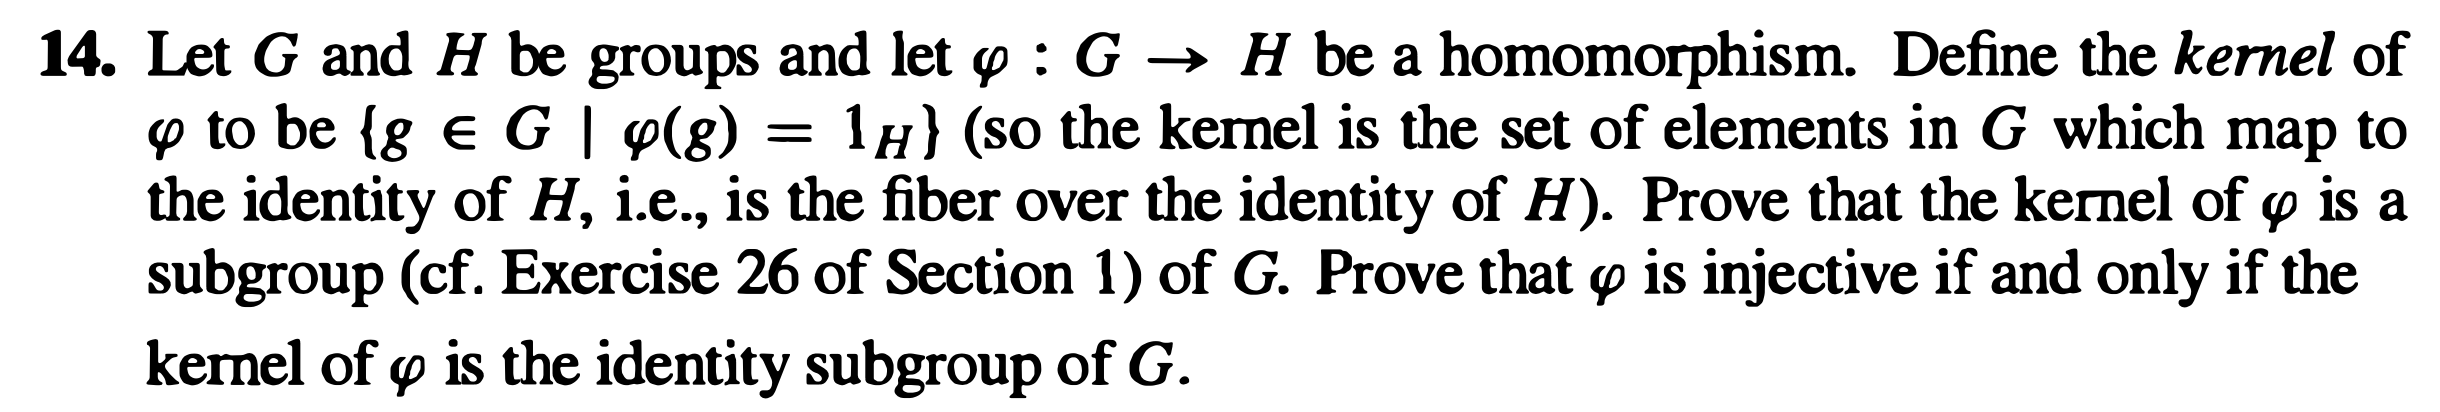
\includegraphics[width=400pt]{img/abstract-algebra--nf--3-b601.png}
\end{mdframed}

\begin{mdframed}

\includegraphics[width=400pt]{img/abstract-algebra--nf--3-b28c.png}
\end{mdframed}


\begin{mdframed}
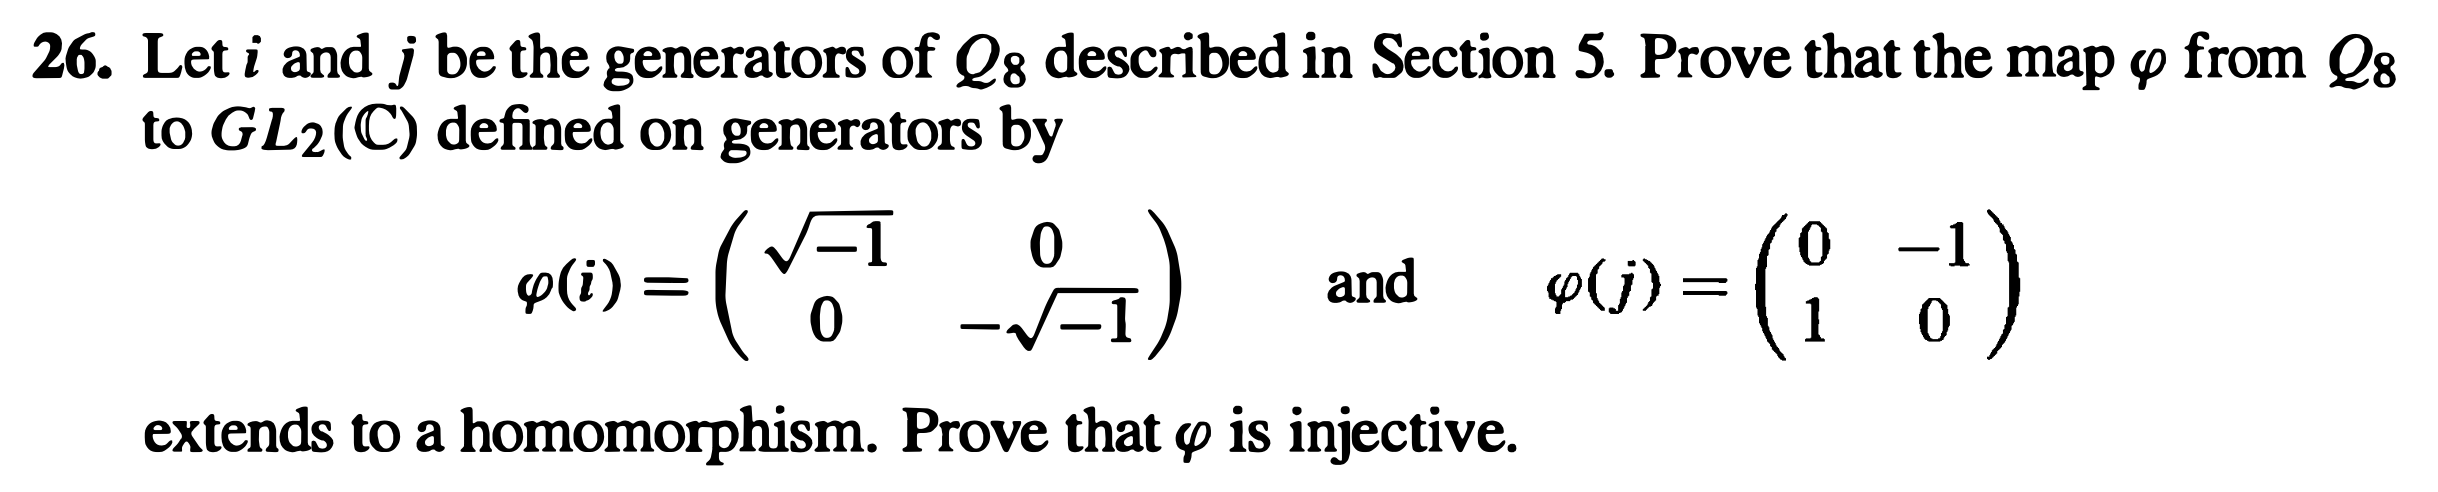
\includegraphics[width=400pt]{img/abstract-algebra--nf--3-1a71.png}
\end{mdframed}
